% This file is part of GUFI, which is part of MarFS, which is released
% under the BSD license.
%
%
% Copyright (c) 2017, Los Alamos National Security (LANS), LLC
% All rights reserved.
%
% Redistribution and use in source and binary forms, with or without modification,
% are permitted provided that the following conditions are met:
%
% 1. Redistributions of source code must retain the above copyright notice, this
% list of conditions and the following disclaimer.
%
% 2. Redistributions in binary form must reproduce the above copyright notice,
% this list of conditions and the following disclaimer in the documentation and/or
% other materials provided with the distribution.
%
% 3. Neither the name of the copyright holder nor the names of its contributors
% may be used to endorse or promote products derived from this software without
% specific prior written permission.
%
% THIS SOFTWARE IS PROVIDED BY THE COPYRIGHT HOLDERS AND CONTRIBUTORS "AS IS" AND
% ANY EXPRESS OR IMPLIED WARRANTIES, INCLUDING, BUT NOT LIMITED TO, THE IMPLIED
% WARRANTIES OF MERCHANTABILITY AND FITNESS FOR A PARTICULAR PURPOSE ARE DISCLAIMED.
% IN NO EVENT SHALL THE COPYRIGHT HOLDER OR CONTRIBUTORS BE LIABLE FOR ANY DIRECT,
% INDIRECT, INCIDENTAL, SPECIAL, EXEMPLARY, OR CONSEQUENTIAL DAMAGES (INCLUDING,
% BUT NOT LIMITED TO, PROCUREMENT OF SUBSTITUTE GOODS OR SERVICES; LOSS OF USE,
% DATA, OR PROFITS; OR BUSINESS INTERRUPTION) HOWEVER CAUSED AND ON ANY THEORY OF
% LIABILITY, WHETHER IN CONTRACT, STRICT LIABILITY, OR TORT (INCLUDING NEGLIGENCE
% OR OTHERWISE) ARISING IN ANY WAY OUT OF THE USE OF THIS SOFTWARE, EVEN IF
% ADVISED OF THE POSSIBILITY OF SUCH DAMAGE.
%
%
% From Los Alamos National Security, LLC:
% LA-CC-15-039
%
% Copyright (c) 2017, Los Alamos National Security, LLC All rights reserved.
% Copyright 2017. Los Alamos National Security, LLC. This software was produced
% under U.S. Government contract DE-AC52-06NA25396 for Los Alamos National
% Laboratory (LANL), which is operated by Los Alamos National Security, LLC for
% the U.S. Department of Energy. The U.S. Government has rights to use,
% reproduce, and distribute this software.  NEITHER THE GOVERNMENT NOR LOS
% ALAMOS NATIONAL SECURITY, LLC MAKES ANY WARRANTY, EXPRESS OR IMPLIED, OR
% ASSUMES ANY LIABILITY FOR THE USE OF THIS SOFTWARE.  If software is
% modified to produce derivative works, such modified software should be
% clearly marked, so as not to confuse it with the version available from
% LANL.
%
% THIS SOFTWARE IS PROVIDED BY LOS ALAMOS NATIONAL SECURITY, LLC AND CONTRIBUTORS
% "AS IS" AND ANY EXPRESS OR IMPLIED WARRANTIES, INCLUDING, BUT NOT LIMITED TO,
% THE IMPLIED WARRANTIES OF MERCHANTABILITY AND FITNESS FOR A PARTICULAR PURPOSE
% ARE DISCLAIMED. IN NO EVENT SHALL LOS ALAMOS NATIONAL SECURITY, LLC OR
% CONTRIBUTORS BE LIABLE FOR ANY DIRECT, INDIRECT, INCIDENTAL, SPECIAL,
% EXEMPLARY, OR CONSEQUENTIAL DAMAGES (INCLUDING, BUT NOT LIMITED TO, PROCUREMENT
% OF SUBSTITUTE GOODS OR SERVICES; LOSS OF USE, DATA, OR PROFITS; OR BUSINESS
% INTERRUPTION) HOWEVER CAUSED AND ON ANY THEORY OF LIABILITY, WHETHER IN
% CONTRACT, STRICT LIABILITY, OR TORT (INCLUDING NEGLIGENCE OR OTHERWISE) ARISING
% IN ANY WAY OUT OF THE USE OF THIS SOFTWARE, EVEN IF ADVISED OF THE POSSIBILITY
% OF SUCH DAMAGE.



\subsubsection{\gufidirindex}
\gufidirindex is used to directly create an index based off of the
contents of a provided directory.

\begin{table} [h]
  \centering
  \begin{tabular}{l|r}
    Flag & Functionality \\\hline
    -h & help manual \\
    -H & Show assigned input values \\
    -n \textless num\_threads\textgreater  & define number of threads to use \\
    -x & pull xattrs from source file-sys into GUFI \\
    -z \textless max\_level\textgreater & maximum level to go down to
  \end{tabular}
  \caption{\label{fig:Flags_for_dir2index} \gufidirindex Flags and Arguments}
\end{table}

\begin{figure} [h]
  \centering
  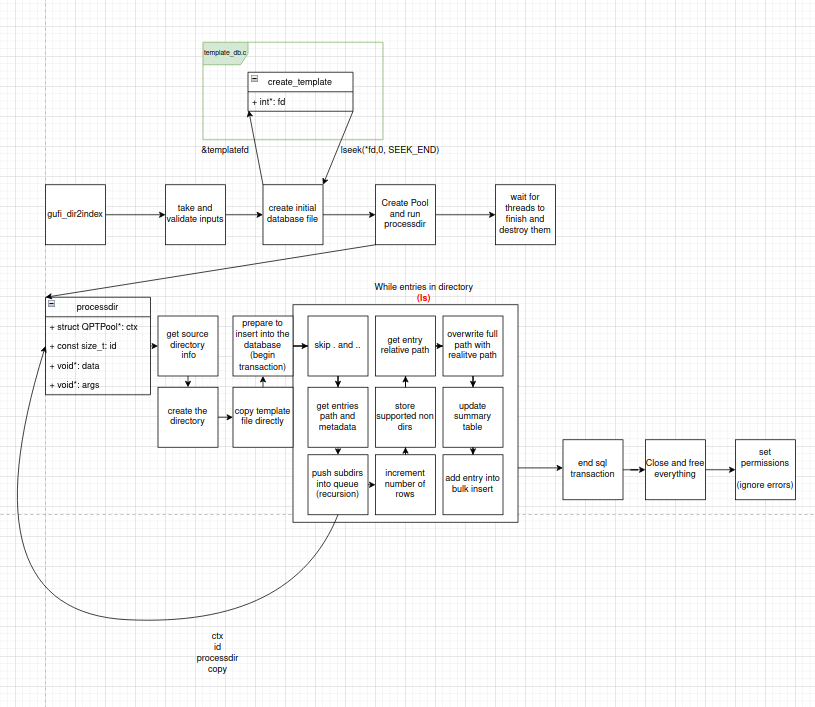
\includegraphics[width=1.0\textwidth]{images/gufi_dir2index.png}
  \caption{\label{fig:gufi_dir2index} \gufidirindex workflow}
\end{figure}

\paragraph{Usage} ~\\
\gufidirindex \texttt{[flags] input\_dir... output\_dir}
